% Options for packages loaded elsewhere
\PassOptionsToPackage{unicode}{hyperref}
\PassOptionsToPackage{hyphens}{url}
%
\documentclass[
  ignorenonframetext,
]{beamer}
\usepackage{pgfpages}
\setbeamertemplate{caption}[numbered]
\setbeamertemplate{caption label separator}{: }
\setbeamercolor{caption name}{fg=normal text.fg}
\beamertemplatenavigationsymbolsempty
% Prevent slide breaks in the middle of a paragraph
\widowpenalties 1 10000
\raggedbottom
\setbeamertemplate{part page}{
  \centering
  \begin{beamercolorbox}[sep=16pt,center]{part title}
    \usebeamerfont{part title}\insertpart\par
  \end{beamercolorbox}
}
\setbeamertemplate{section page}{
  \centering
  \begin{beamercolorbox}[sep=12pt,center]{part title}
    \usebeamerfont{section title}\insertsection\par
  \end{beamercolorbox}
}
\setbeamertemplate{subsection page}{
  \centering
  \begin{beamercolorbox}[sep=8pt,center]{part title}
    \usebeamerfont{subsection title}\insertsubsection\par
  \end{beamercolorbox}
}
\AtBeginPart{
  \frame{\partpage}
}
\AtBeginSection{
  \ifbibliography
  \else
    \frame{\sectionpage}
  \fi
}
\AtBeginSubsection{
  \frame{\subsectionpage}
}
\usepackage{amsmath,amssymb}
\usepackage{lmodern}
\usepackage{iftex}
\ifPDFTeX
  \usepackage[T1]{fontenc}
  \usepackage[utf8]{inputenc}
  \usepackage{textcomp} % provide euro and other symbols
\else % if luatex or xetex
  \usepackage{unicode-math}
  \defaultfontfeatures{Scale=MatchLowercase}
  \defaultfontfeatures[\rmfamily]{Ligatures=TeX,Scale=1}
\fi
\usetheme[]{Madrid}
\usecolortheme{rose}
% Use upquote if available, for straight quotes in verbatim environments
\IfFileExists{upquote.sty}{\usepackage{upquote}}{}
\IfFileExists{microtype.sty}{% use microtype if available
  \usepackage[]{microtype}
  \UseMicrotypeSet[protrusion]{basicmath} % disable protrusion for tt fonts
}{}
\makeatletter
\@ifundefined{KOMAClassName}{% if non-KOMA class
  \IfFileExists{parskip.sty}{%
    \usepackage{parskip}
  }{% else
    \setlength{\parindent}{0pt}
    \setlength{\parskip}{6pt plus 2pt minus 1pt}}
}{% if KOMA class
  \KOMAoptions{parskip=half}}
\makeatother
\usepackage{xcolor}
\newif\ifbibliography
\setlength{\emergencystretch}{3em} % prevent overfull lines
\providecommand{\tightlist}{%
  \setlength{\itemsep}{0pt}\setlength{\parskip}{0pt}}
\setcounter{secnumdepth}{-\maxdimen} % remove section numbering
\newlength{\cslhangindent}
\setlength{\cslhangindent}{1.5em}
\newlength{\csllabelwidth}
\setlength{\csllabelwidth}{3em}
\newlength{\cslentryspacingunit} % times entry-spacing
\setlength{\cslentryspacingunit}{\parskip}
\newenvironment{CSLReferences}[2] % #1 hanging-ident, #2 entry spacing
 {% don't indent paragraphs
  \setlength{\parindent}{0pt}
  % turn on hanging indent if param 1 is 1
  \ifodd #1
  \let\oldpar\par
  \def\par{\hangindent=\cslhangindent\oldpar}
  \fi
  % set entry spacing
  \setlength{\parskip}{#2\cslentryspacingunit}
 }%
 {}
\usepackage{calc}
\newcommand{\CSLBlock}[1]{#1\hfill\break}
\newcommand{\CSLLeftMargin}[1]{\parbox[t]{\csllabelwidth}{#1}}
\newcommand{\CSLRightInline}[1]{\parbox[t]{\linewidth - \csllabelwidth}{#1}\break}
\newcommand{\CSLIndent}[1]{\hspace{\cslhangindent}#1}
\renewcommand{\bibfont}{\small}
\ifLuaTeX
  \usepackage{selnolig}  % disable illegal ligatures
\fi
\IfFileExists{bookmark.sty}{\usepackage{bookmark}}{\usepackage{hyperref}}
\IfFileExists{xurl.sty}{\usepackage{xurl}}{} % add URL line breaks if available
\urlstyle{same} % disable monospaced font for URLs
\hypersetup{
  pdftitle={Collective risk},
  pdfauthor={Ignacio Gómez, Gonzalo Pato, Gonzalo Prats},
  hidelinks,
  pdfcreator={LaTeX via pandoc}}

\title{Collective risk}
\author{Ignacio Gómez, Gonzalo Pato, Gonzalo Prats}
\date{April 2023}
\institute{Simulation in Prob and Stats BSc AMC at UC3M}

\begin{document}
\frame{\titlepage}

\begin{frame}{Contents}
\protect\hypertarget{contents}{}
\begin{itemize}
\tightlist
\item
  \textbf{Introduction}
\item
  \textbf{The project}
\item
  \textbf{Results}
\item
  \textbf{Conclusions}
\item
  \textbf{References}
\end{itemize}
\end{frame}

\begin{frame}{Introduction}
\protect\hypertarget{introduction}{}
\begin{itemize}
\tightlist
\item
  Goal:

  \begin{itemize}
  \tightlist
  \item
    Compute the probability that the capital of an insurance company
    remains positive during a given time period
  \end{itemize}
\item
  Data:

  \begin{itemize}
  \tightlist
  \item
    Premium: \(a\)
  \item
    Claims rate: \(Poisson (\lambda)\)
  \item
    Premium amount: \(Pareto (2.5, 100)\)
  \item
    Enrollment rate: \(Poisson(\nu)\)
  \item
    Departure rate: \(Exp(\mu)\)
  \item
    Initial capital: \(c_0\)
  \end{itemize}
\end{itemize}
\end{frame}

\begin{frame}{Introduction}
\protect\hypertarget{introduction-1}{}
So in general, the capital of the company at any time \(t\) will be:

\[C(t) = c_0 + at(n_0+N_A(t)-N_D(t)) - \sum_{j=1}^{N_C(t)} X_j\]

where:

\begin{itemize}
\item $N_A(t)$ is the number of clients that arrive by time $t$
\item $N_D(t)$ is the number of clients that leave by time $t$
\item $N_C(t)$ is the number of claims that arrive by time $t$
\item $X_j$ is the amount of the $j$-th claim
\item $n(t)$ is the number of clients at time $t$.
\end{itemize}
\end{frame}

\begin{frame}{The project}
\protect\hypertarget{the-project}{}
\begin{center}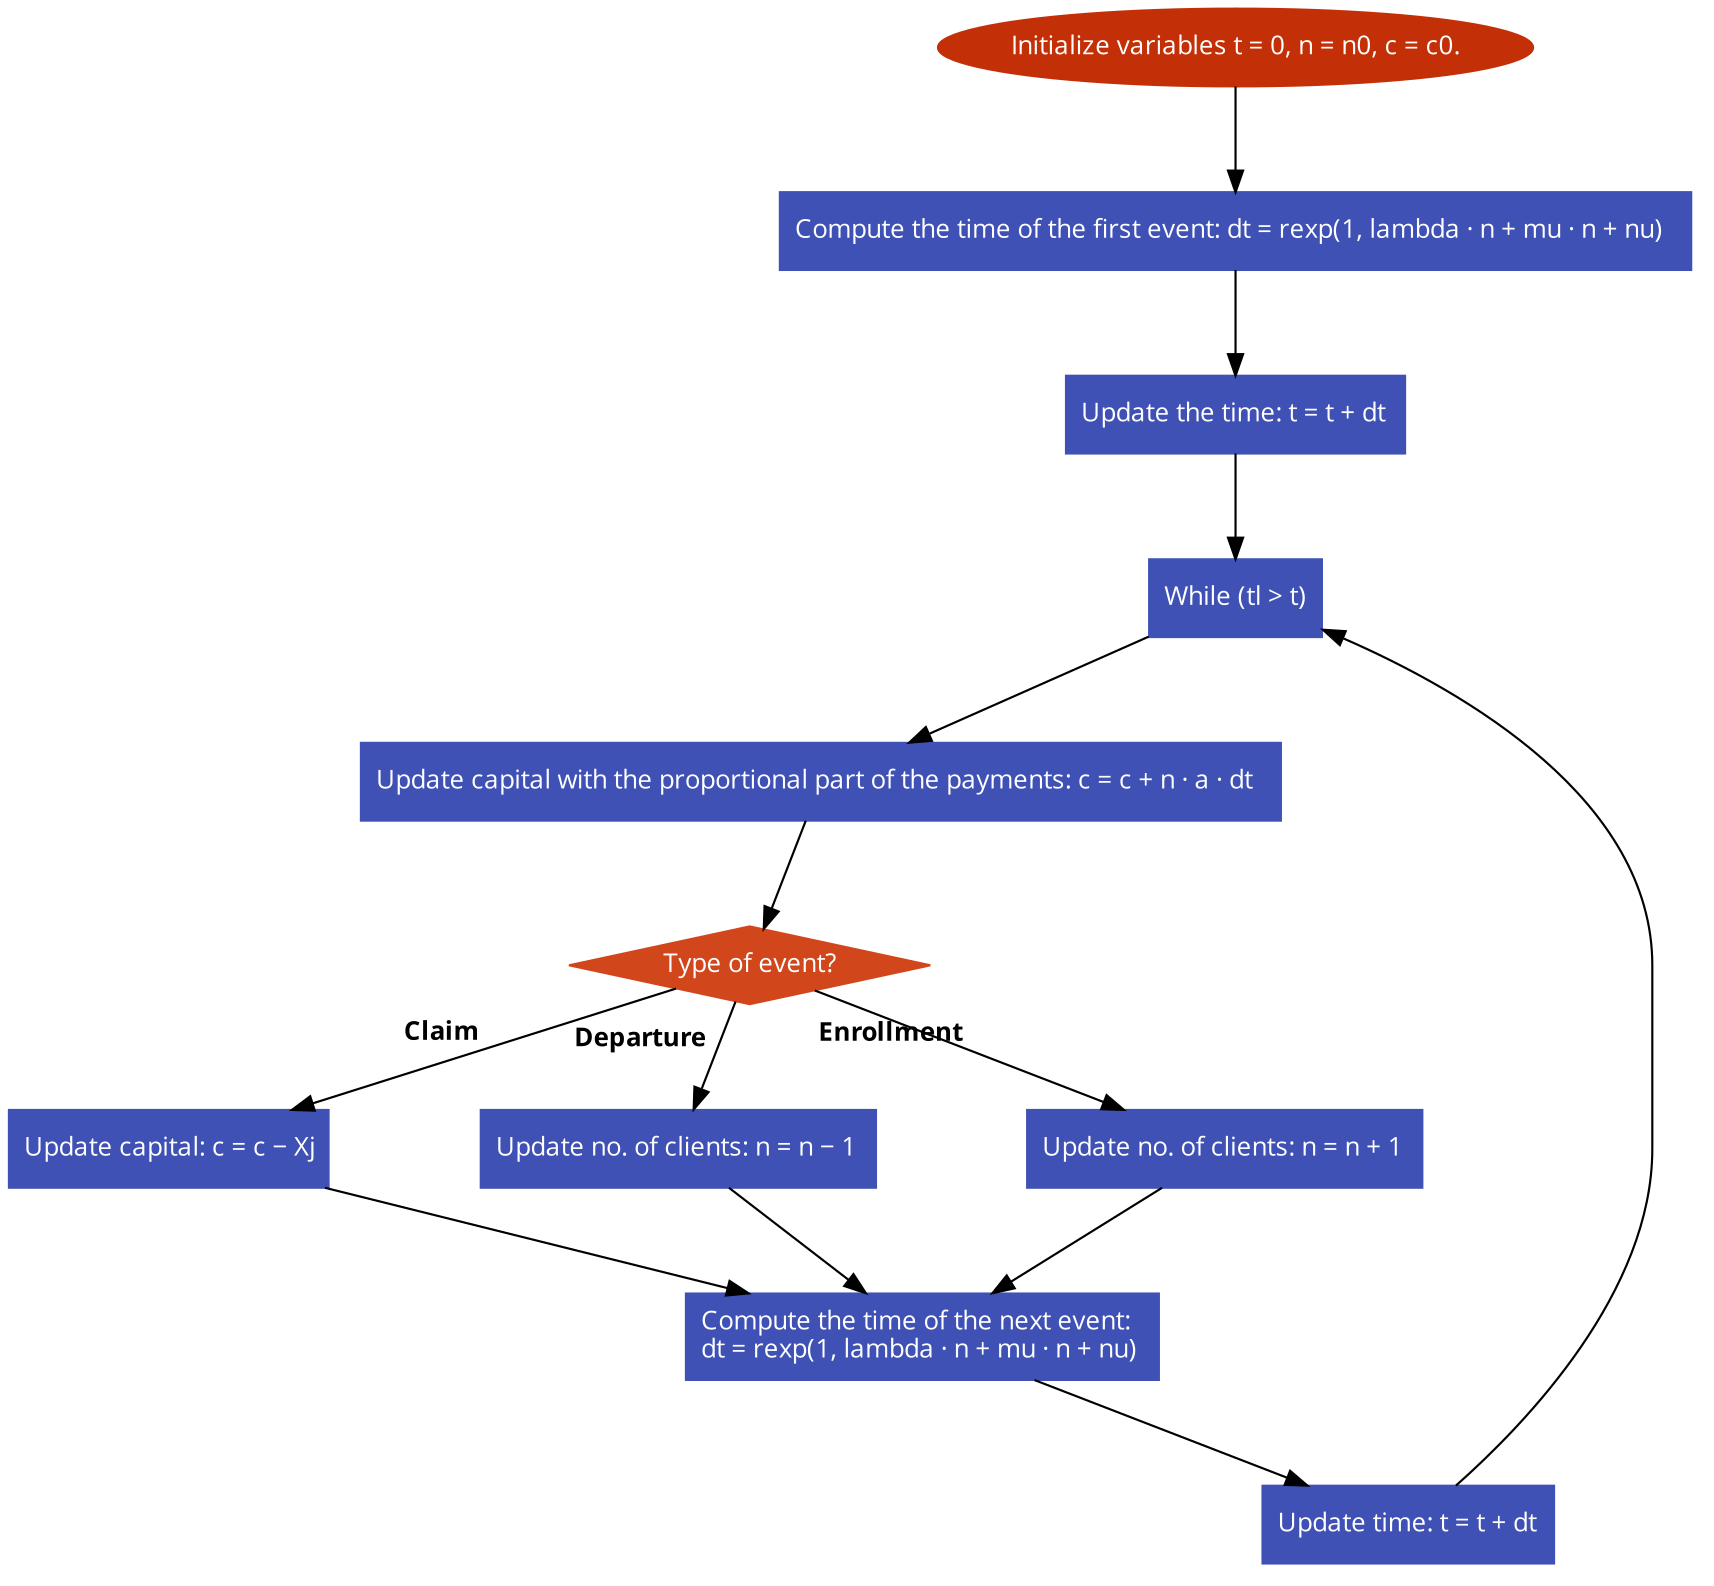
\includegraphics[width=0.7\linewidth]{flux} \end{center}
\end{frame}

\begin{frame}{Results}
\protect\hypertarget{results}{}
We used 2 different approaches for this problem

\begin{itemize}
\item A discrete event simulation algorithm we developed
\item An improved version of our algorithm using antithetic variables to reduce the variance
\end{itemize}

These were the results for \(c_0 = 1000\), \(n_0 = 100\), \(a = 100\),
\(tl = 100\), \(\lambda = 0.1\), \(\mu = 0.1\), \(\nu = 0.1\) and
\(MC = 10000\):

\begin{center}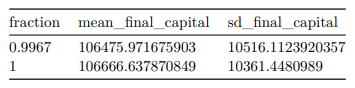
\includegraphics[width=0.8\linewidth]{results_table_comparison} \end{center}
\end{frame}

\begin{frame}{Results}
\protect\hypertarget{results-1}{}
These graphs show both the convergence of the mean of the final capitals
in terms of the number of simulations and the density of the final
capitals. Note that the color red indicates the antithetic variables
approach

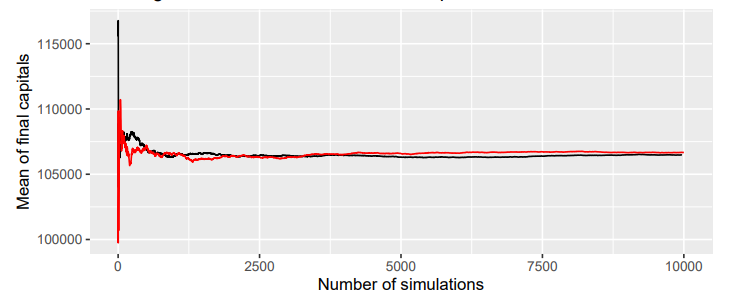
\includegraphics[width=0.45\linewidth]{mean_final_cap}
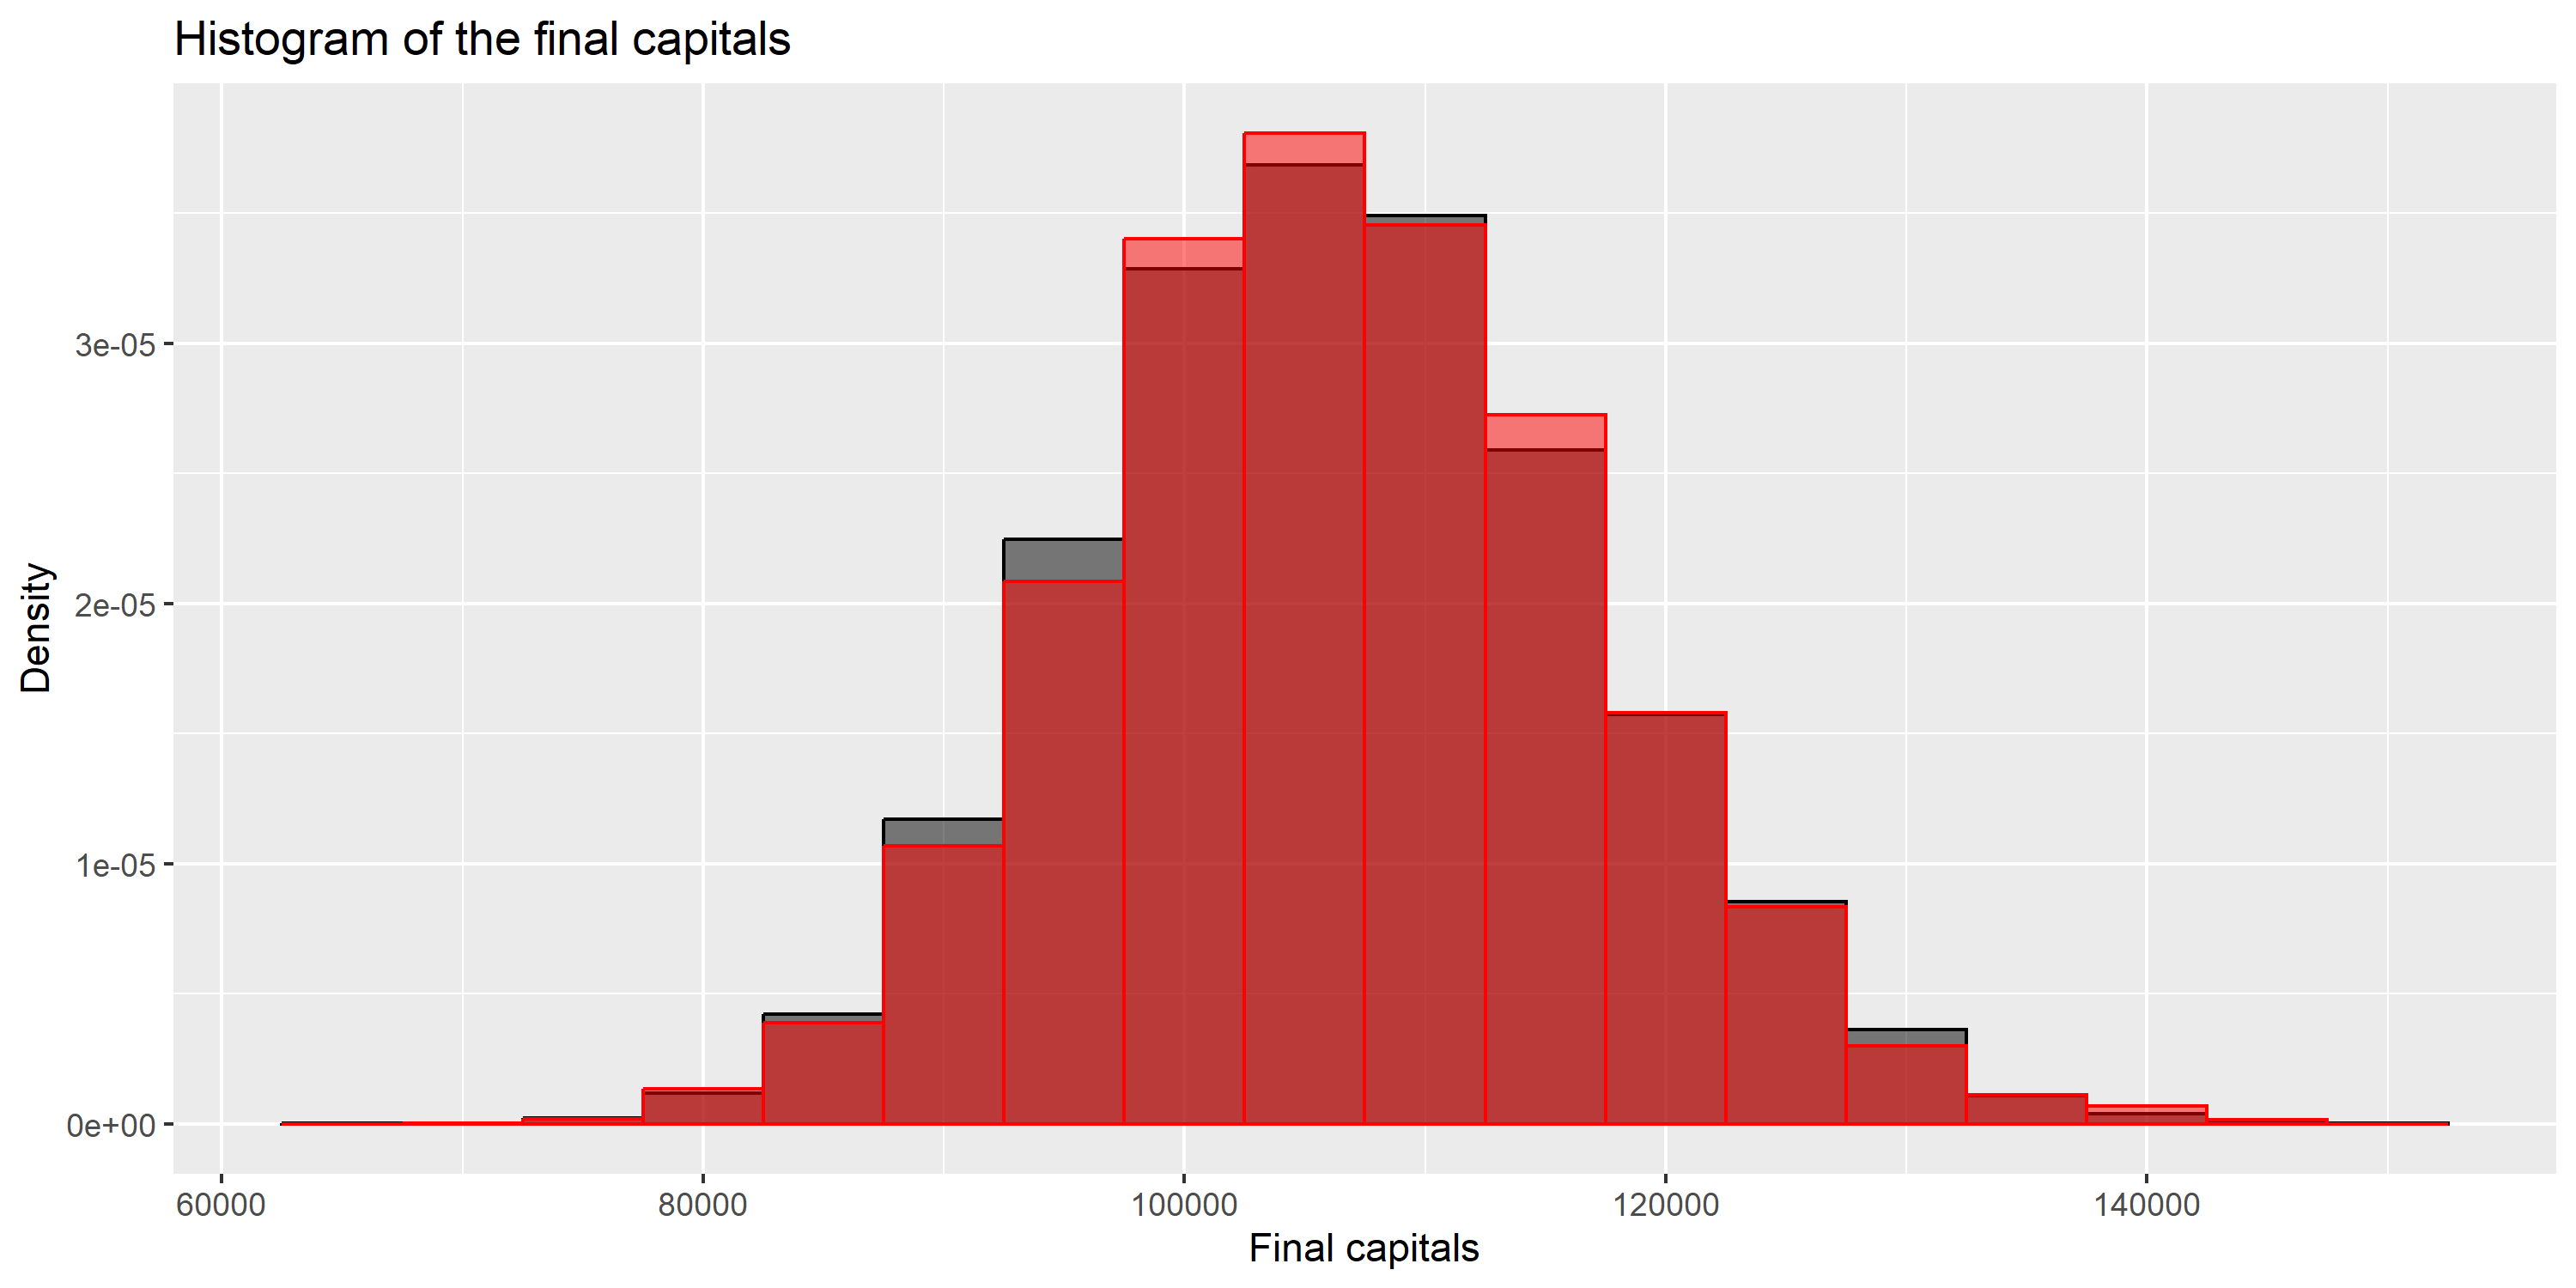
\includegraphics[width=0.45\linewidth]{densities_final_caps}
\end{frame}

\begin{frame}{Conclusions}
\protect\hypertarget{conclusions}{}
About the results, how the difficulties were solved, and possible
alternative approaches. Keep the focus, the conclusions must be as brief
as possible.
\end{frame}

\begin{frame}{References}
\protect\hypertarget{references}{}
\hypertarget{refs}{}
\begin{CSLReferences}{1}{0}
\leavevmode\vadjust pre{\hypertarget{ref-Unit2}{}}%
Cascos, Ignacio. 2023a. {``Lecture Notes 2. Simulating Random Variables
and Vectors.''} Aula Global UC3M.

\leavevmode\vadjust pre{\hypertarget{ref-Unit4}{}}%
---------. 2023b. {``Lecture Notes 4. Efficiency Improvement
Techniques.''} Aula Global UC3M.

\leavevmode\vadjust pre{\hypertarget{ref-Kaas2008}{}}%
{``Collective Risk Models.''} 2008. In \emph{Modern Actuarial Risk
Theory: Using r}, 41--86. Berlin, Heidelberg: Springer Berlin
Heidelberg. \url{https://doi.org/10.1007/978-3-540-70998-5_3}.

\leavevmode\vadjust pre{\hypertarget{ref-ggplot22016}{}}%
Wickham, Hadley. 2016. \emph{Ggplot2: Elegant Graphics for Data
Analysis}. Springer-Verlag New York.
\url{https://ggplot2.tidyverse.org}.

\leavevmode\vadjust pre{\hypertarget{ref-R-ggplot2}{}}%
Wickham, Hadley, Winston Chang, Lionel Henry, Thomas Lin Pedersen,
Kohske Takahashi, Claus Wilke, Kara Woo, Hiroaki Yutani, and Dewey
Dunnington. 2023. \emph{Ggplot2: Create Elegant Data Visualisations
Using the Grammar of Graphics}.
\url{https://CRAN.R-project.org/package=ggplot2}.

\leavevmode\vadjust pre{\hypertarget{ref-R-dplyr}{}}%
Wickham, Hadley, Romain François, Lionel Henry, Kirill Müller, and Davis
Vaughan. 2023. \emph{Dplyr: A Grammar of Data Manipulation}.
\url{https://CRAN.R-project.org/package=dplyr}.

\leavevmode\vadjust pre{\hypertarget{ref-R-cowplot}{}}%
Wilke, Claus O. 2020. \emph{Cowplot: Streamlined Plot Theme and Plot
Annotations for Ggplot2}. \url{https://wilkelab.org/cowplot/}.

\leavevmode\vadjust pre{\hypertarget{ref-knitr2014}{}}%
Xie, Yihui. 2014. {``Knitr: A Comprehensive Tool for Reproducible
Research in {R}.''} In \emph{Implementing Reproducible Computational
Research}, edited by Victoria Stodden, Friedrich Leisch, and Roger D.
Peng. Chapman; Hall/CRC.

\leavevmode\vadjust pre{\hypertarget{ref-knitr2015}{}}%
---------. 2015. \emph{Dynamic Documents with {R} and Knitr}. 2nd ed.
Boca Raton, Florida: Chapman; Hall/CRC. \url{https://yihui.org/knitr/}.

\leavevmode\vadjust pre{\hypertarget{ref-R-knitr}{}}%
---------. 2023. \emph{Knitr: A General-Purpose Package for Dynamic
Report Generation in r}. \url{https://yihui.org/knitr/}.

\end{CSLReferences}
\end{frame}

\end{document}
